\documentclass[sigconf]{acmart}

%appendix setup
\usepackage{booktabs} % For formal tables
\usepackage[titletoc,toc,title]{appendix}

%note setup
\usepackage{xargs} 
\usepackage{xcolor}
\usepackage[colorinlistoftodos,prependcaption,textsize=tiny]{todonotes}
\newcommandx{\note}[2][1=]{\todo[linecolor=red,backgroundcolor=red!25,bordercolor=red,#1]{#2}}


% Copyright
%\setcopyright{none}
%\setcopyright{acmcopyright}
%\setcopyright{acmlicensed}
\setcopyright{rightsretained}
%\setcopyright{usgov}
%\setcopyright{usgovmixed}
%\setcopyright{cagov}
%\setcopyright{cagovmixed}


% DOI
%\acmDOI{10.475/123_4}

% ISBN
%\acmISBN{123-4567-24-567/08/06}

%Conference
\acmConference[COMO'17]{ACM RecSys conference}{August 2017}{Como, Italy} 
%\acmYear{2017}
%\copyrightyear{2016}

%\acmPrice{15.00}


\begin{document}
\title{Group Recommendation}
%\titlenote{Produces the permission block, and copyright information}
\subtitle{Using Rank Aggregation}
%\subtitlenote{The full version of the author's guide is available as \texttt{acmart.pdf} document}


\author{Lukas Nic Dalgaard}
%\authornote{}
%\orcid{}
\affiliation{%
  \institution{Department of Computer Science Aalborg University}
  \streetaddress{Selma Lagerl\"{o}fs Vej 300}
  \city{Aalborg East} 
  \state{Denmark} 
  \postcode{9220}
}
\email{lnda12@student.aau.dk}

\author{Lasse Drustrup Christensen}
%\authornote{}
\affiliation{%
  \institution{Department of Computer Science Aalborg University}
  \streetaddress{Selma Lagerl\"{o}fs Vej 300}
  \city{Aalborg East} 
  \state{Denmark} 
  \postcode{9220}
}
\email{ldch11@student.aau.dk}

\author{Peter Dolog}
%\authornote{}
\affiliation{%
  \institution{Department of Computer Science Aalborg University}
  \streetaddress{Selma Lagerl\"{o}fs Vej 300}
  \city{Aalborg East} 
  \state{Denmark} 
  \postcode{9220}
}
\email{dolog@cs.aau.dk}



% The default list of authors is too long for headers}
%\renewcommand{\shortauthors}{B. Trovato et al.}


\begin{abstract}
Make an abstract of our article here.\footnote{This is an abstract footnote}
\end{abstract}

%
% The code below should be generated by the tool at
% http://dl.acm.org/ccs.cfm
% Please copy and paste the code instead of the example below. 
%

%CCS CONCEPTS don't know what it is for out commented 
\iffalse
\begin{CCSXML}
<ccs2012>
 <concept>
  <concept_id>10010520.10010553.10010562</concept_id>
  <concept_desc>Computer systems organization~Embedded systems</concept_desc>
  <concept_significance>500</concept_significance>
 </concept>
 <concept>
  <concept_id>10010520.10010575.10010755</concept_id>
  <concept_desc>Computer systems organization~Redundancy</concept_desc>
  <concept_significance>300</concept_significance>
 </concept>
 <concept>
  <concept_id>10010520.10010553.10010554</concept_id>
  <concept_desc>Computer systems organization~Robotics</concept_desc>
  <concept_significance>100</concept_significance>
 </concept>
 <concept>
  <concept_id>10003033.10003083.10003095</concept_id>
  <concept_desc>Networks~Network reliability</concept_desc>
  <concept_significance>100</concept_significance>
 </concept>
</ccs2012>  
\end{CCSXML}

\ccsdesc[500]{Computer systems organization~Embedded systems}
\ccsdesc[300]{Computer systems organization~Redundancy}
\ccsdesc{Computer systems organization~Robotics}
\ccsdesc[100]{Networks~Network reliability}
\fi

% We no longer use \terms command
%\terms{Theory}

\keywords{Group Recommendation, ...}


\maketitle

\section{Introduction}
Many of the decisions we make are based on recommendation, from either people we know or a recommender system which knows our preferences, due to the amount of information overload we are exposed to. The recommendations, or more specific on our case the recommender system, can be a help to reduce the amount of information we are presented with to a manageable level and hereby ease the decision making without forcing a decision on us. 

The problem with the traditional recommender systems is that it typically make recommendations specifically to one person put often these decisions needs to be taken in a social context. Some scenarios where this could be the case is for example selecting a film to watch from the seemingly endless ones available on the streaming services, Which restaurant you should go to, or which vacation destination suits you best. 

One for the problem regarding taking the social context into consideration is that the recommender have to strive for consensus between the people it recommends to. From here, we will reference to this problem as making a group recommendation.

%Different methods for group recommendations 
When making group recommendations there are two main approach namely profile aggregation and recommendation aggregation.\note{cite, page 516 in rec. book} The idea behind profile aggregation is to aggregate the users preferences into a group profile and make aggregations based on that profile. The recommendation aggregation method aggregates the recommendations for the individual users into one aggregation that should fit the groups preferences. In this paper we have chosen to focus on the latter, as we want to make the method work for shifting groups and we deem this approach to fit this case best. \note{find source or fitting argument}

%Describe the approach of using top-k lists 
As we are going to aggregate the users recommendations we have chosen to only to focus at the top-k part of their recommendations and return a top-k lists as a result. Furthermore, the top-k lists will be ranked with the highest rated item at first position on the list. Throughout the paper we have worked with a $k$ of size 10. 

Working with partial lists, which ranked top-k lists are, we have selected three types of aggregation list which have shown good results when used for aggregating search engine results within the information retrieval domain. The methods we are using is Borda Count, Markov Chain, and Spearman's Footrule. We also implemented an Average aggregation method as a control algorithm. 

%Problem regarding evaluation of the aggregation results
Having the group recommendations we are faced with the challenge of evaluating the result as there are no dataset supplying us with a ground truth. Alternatively we use some different equality measures in order to verify the results. 
\note{extend this}


%Lukas
%As it is no longer of question of should the computers be involved when humans make decisions but how.

%Recommender systems can strengthen decision making without taking away the final choice from humans. This opens the 

%For making a decision, Edwards et al provide a 19 step guide for picking the option with the highest utility, and they argue that the problem for a user would be in picking from among the many options presented, also known as information overload\cite{Edwards2001}.

%Recommender systems deal with reducing the problem for a user to a manageable amount of choices. Given a user's preferences, a good recommender system can narrow down the number of choices to a manageable level.

%However when the problem area is expanded to include multiple users in need of a single choice, the problem area is two-fold, as the many individual preferences must be aligned into that of a single recommendation.

%The recommender system is doubly challenged as while a single user can navigate the given recommendations and reflect on each item for the best optimal choice, a group will have a hard time making insightful decisions about items they lack the shared information of the group to comment on.
\note{Lukas: Possible direction for the introduction?}

\subsection{Composition of a Group Recommender}
As we take the aspect of aggregating recommendations the group recommendation system will consist of two parts namely an individual recommender and an aggregation method. \note{need some extension and probably an illustration}

\subsection{Thesis}\note{Placeholder title}
How can we by supplying a rank aggregation method with an array ranked top-k lists $\tau_1, ... , \tau_u$, where $u$ is the number of group members, get a recommendation performing better than an average aggregation. \note{this should probably be more specific and technical}

\subsection{Structure of the Paper}
The structure of the paper is as follows. In Section \ref{sec:preliminaries} contains the preliminaries including the measures used during the evaluation. Section \ref{sec:aggregations} describes the aggregation methods used. In Section \ref{sec:evaluation} the performances of the aggregation methods are documented. Section \ref{sec:discussion} we discuss the results of the evaluation and in Section \ref{sec:conclusion} we will present our conclusion and some future work to be done.
\section{Related Work}
%Context
In their work on aggregation of search queries, Dwork et al presented 4 Markov Chain(MC) methods.

To Dwork et Al, the idea of MC that the current state impacts future states were useful to get a better aggregation and provide a better interplay between candidates by comparing all candidates against each other. 

%Enhancement of other heuristics
It was their belief that this property of MC provided a natural extension to common aggregation methods such as Borda Count\note{First mention? BC?}.

Of the four methods presented, \MC managed to achieve some of the best results when scored on distance measures such as Kendall distance or Spearman's footrule, so of the four \MC will be our focus in this article.\cite{rank:aggregation}
\section{Methodology}

\begin{frame}
     \begin{center}
     	\huge Methodology
     \end{center}
\end{frame}

\begin{frame}
	\frametitle{Something}
	Bla bla bla  
\end{frame}
\section{Recommendations}\label{sec:recommendations}
In order to validate the proposed method we have used several different measures.

\begin{frame}[t]
\frametitle{Borda Count}
\begin{columns}
\begin{column}{0.5\textwidth}
\begin{align*}
	bc(i) = \sum_{u\in U} \tau_u(i)
\end{align*}
\small
\begin{align*}
	bc(A) = \tau_{u_1}(A) + \tau_{u_2}(A) + \tau_{u_3}(A) + \tau_{u_4}(A)
\end{align*}
\normalsize
\begin{align*}
	bc(A) = 5 + 4 + 2 + 3 = 14
\end{align*}

\end{column}
\begin{column}{0.5\textwidth}
\small
\vspace{-0.5cm}
\begin{table}
\captionsetup{font=footnotesize}
\begin{tabular}{|l|lllll|} \hline
Rank  & 1 & 2 & 3 & 4 & 5 \\\hline
$u_1$ & A & B & C & D & E \\
$u_2$ & C & D & F & A & E \\
$u_3$ & E & A & G & B & D \\
$u_4$ & G & H & A & E & F\\\hline
\end{tabular}
\caption{Top-k list of a group with 4 users}
\end{table}

\vspace{-1cm}
\begin{table}
\begin{tabular}{|l|llllllll|}\hline
      & A & B & C & D & E & F & G & H \\\hline
$u_1$ & 5 & 4 & 3 & 2 & 1 & 0 & 0 & 0 \\
$u_2$ & 2 & 0 & 5 & 4 & 1 & 3 & 0 & 0 \\
$u_3$ & 4 & 2 & 0 & 1 & 5 & 0 & 3 & 0 \\
$u_4$ & 3 & 0 & 0 & 0 & 2 & 1 & 5 & 4 \\\hline
Sum	  & 14& 6 & 8 & 7 & 9 & 4 & 8 & 4 \\\hline
\end{tabular}
\caption{Borda Count scores}
\end{table}
\normalsize
\end{column}
\end{columns}
\begin{table}
\begin{tabular}{llllll}
Recommendations: & A & E & C & G & D
\end{tabular}
\end{table}
\end{frame}

%
%\begin{columns}
%\begin{column}{0.5\textwidth}
%
%\end{column}
%\begin{column}{0.5\textwidth}
%
%\end{column}
%\end{columns}
\subsection{Markov Chain}\label{sec:markovchain}
The proposed Markov Chain method by Dwork et Al, \MC is a generalization of the Copeland Method\note{find cite for this}, where a winner is the candidate which wins the most pairwise contests\citep{rank:aggregation}.

The concept behind building the list of recommendations works by explicitly finding the transition matrix. For \MC, the states are connected to other states that wins per the Copeland method. Then we can iterate through the set, and note who performs best to make the transition matrix. Using the power set on the transition matrix we can find the stationary probability distribution to aggregate the candidates.

The \MC state space corresponds to a set of all the items ranked. The corresponding transition matrix for \MC will have an equal chance of transitioning to any other state that can beat it in a majority of pairwise contests.

Given partial lists $\tau_1,...,\tau_k$, collectively known as $\tau$, with rankings of items, and the state space, $S$, of \MC corresponding to the set of all items ranked in those partial lists. If the current state is item $i$ we can transition to uniformly picked state $j \in S$ where $j$ is ranked higher than item $i$ on a majority of lists in $\tau$ which ranked both $i$ and $j$. Otherwise, we stay in state $i$.

%Non-strict markov chain
\MC as presented by Dwork et al is used on metasearch and aggregating query results, whereas we work in the recommendation domain. To better suit our domain, we make a small adjustment to the method. For search engine comparison, partial lists might not contain both items needed for a pairwise comparison, so in the event of only one item being on the list, it is unknown if the other search engines have ranked the item or not, so Dwork et al restrict themselves to the pairwise comparisons available, and rely on the connectivity in the chain to correct any outcomes.

For our domain we have estimated the rankings giving us a top-k of a full list. So we follow this line of thinking for partial lists containing neither of the items, as the highest rank is not available. However, if the partial list contains one of the items, it wins that pairwise contest, as the losing item is known to be somewhere down the list.

%$p_{ij} = Pr(X_{n+1} = \sum_{l=1}^{k} \tau_l(i) < \tau_l(j) | X_n = \sum_{l=1}^{k} \tau_l(i) > \tau_l(j) )$

%Strict markov chain
%For completeness, we also tested a stricter interpretation of \MC where only the majority winners with both items present were considered.
\subsection{Spearman Footrule}\label{sec:spearmanfootrule}
\section{Results}

\begin{frame}
     \begin{center}
     	\huge Results 
     \end{center}
\end{frame}

\begin{frame}
	\frametitle{Methodology}
	The setup of the new test is the same as the previous tests
	\begin{itemize}
		\item The exact same random generated groups as in the previous tests
		\item Groups of the sizes 4, 8, 12, 16, 20, and 40
		\item There are 1000 groups of each size
		\item The preferences looked at is the top 10
	\end{itemize}
\end{frame}

\begin{frame}
\frametitle{Group Size 4}
\begin{figure}[h]
\centering
\begin{minipage}{.46\textwidth}\centering
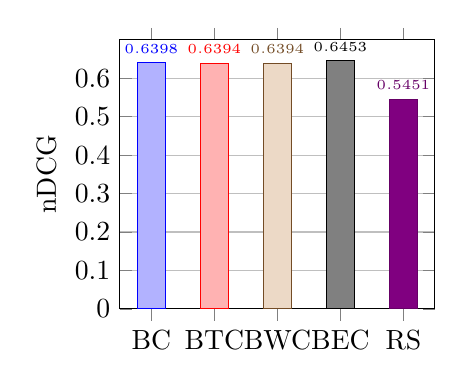
\begin{tikzpicture}
 \begin{axis}[
 	height=5cm,
 	width=4cm,
 	ybar =-10pt,
 	x = .8cm,
 	ymin=0.0, 
 	ymax=0.70,
 	ytick = {0, 0.1,0.2,0.3,...,0.70},
 	scaled y ticks = false,
	enlarge x limits ={abs=.4cm},
	nodes near coords,
    every node near coord/.append style={font=\tiny,/pgf/number format/.cd,precision=4},
 	ylabel={nDCG},
	xtick={0,1,2,3,4},  % NEW BIT
	xticklabels={BC, BTC, BWC, BEC, RS},
	%legend style={at={(0.5,-0.1)},
	%anchor=north,legend columns=-1},
	ymajorgrids = true,]

		\addplot coordinates {(0,0.6398)};    
		\addplot coordinates {(1,0.6394)};    
		\addplot coordinates {(2,0.6394)};    
		\addplot coordinates {(3,0.6453)};    
		\addplot coordinates {(4,0.5451)};
        %\legend{BC, BTC, BWC, BEC, Random}
     \end{axis}
\end{tikzpicture}
\end{minipage}
\begin{minipage}{.46\textwidth}\centering
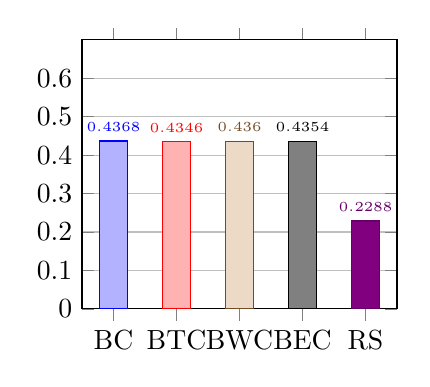
\begin{tikzpicture}
 \begin{axis}[
 	height=5cm,
 	ybar =-10pt,
 	x = .8cm,
 	ymin=0.0, 	
 	ymax=0.70,
 	ytick = {0,0.1,0.20,0.3,...,0.70},
	enlarge x limits ={abs=.4cm},
	nodes near coords,
    every node near coord/.append style={font=\tiny,/pgf/number format/.cd,precision=4},
	xtick={0,1,2,3,4},  % NEW BIT
	xticklabels={BC, BTC, BWC, BEC, RS},
	%legend style={at={(0.5,-0.1)},
	%anchor=north,legend columns=-1},
	ymajorgrids = true,]

		\addplot coordinates {(0,0.4368)};    
		\addplot coordinates {(1,0.4346)};    
		\addplot coordinates {(2,0.436)};    
		\addplot coordinates {(3,0.4354)};    
		\addplot coordinates {(4,0.2288)};
        %\legend{BC, BTC, BWC, BEC, Random}
     \end{axis}
\end{tikzpicture}
\end{minipage}
\end{figure}
\end{frame}

\begin{frame}
\frametitle{Group Size 12}
\begin{figure}[h]
\centering
\begin{minipage}{.46\textwidth}\centering
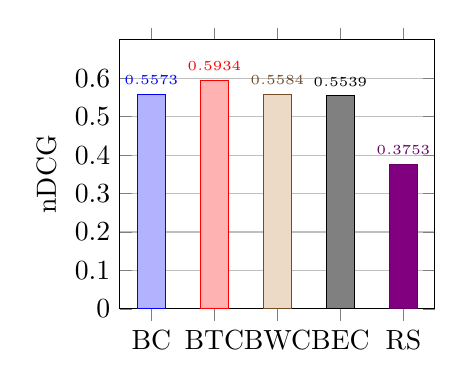
\begin{tikzpicture}
 \begin{axis}[
 	height=5cm,
 	width=4cm,
 	ybar =-10pt,
 	x = .8cm,
 	ymin=0.00, 
 	ymax=0.70,
 	ytick = {0,0.1,0.2,0.3,...,0.70},
 	scaled y ticks = false,
	enlarge x limits ={abs=.4cm},
	nodes near coords,
    every node near coord/.append style={font=\tiny,/pgf/number format/.cd,precision=4},
 	ylabel={nDCG},
	xtick={0,1,2,3,4},  % NEW BIT
	xticklabels={BC, BTC, BWC, BEC, RS},
	%legend style={at={(0.5,-0.1)},
	%anchor=north,legend columns=-1},
	ymajorgrids = true,]

		\addplot coordinates {(0,0.5573)};    
		\addplot coordinates {(1,0.5934)};    
		\addplot coordinates {(2,0.5584)};    
		\addplot coordinates {(3,0.5539)};    
		\addplot coordinates {(4,0.3753)};
        %\legend{BC, BTC, BWC, BEC, Random}
     \end{axis}
\end{tikzpicture}
\end{minipage}
\begin{minipage}{.46\textwidth}\centering
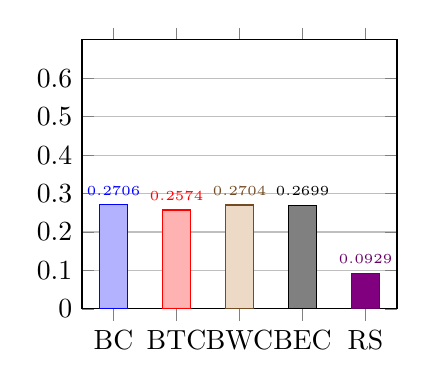
\begin{tikzpicture}
 \begin{axis}[
 	height=5cm,
 	ybar =-10pt,
 	x = .8cm,
 	ymin=0.0, 	
 	ymax=0.70,
 	ytick = {0,0.1,0.20,0.3,...,0.70},
	enlarge x limits ={abs=.4cm},
	nodes near coords,
    every node near coord/.append style={font=\tiny,/pgf/number format/.cd,precision=4},
	xtick={0,1,2,3,4},  % NEW BIT
	xticklabels={BC, BTC, BWC, BEC, RS},
	%legend style={at={(0.5,-0.1)},
	%anchor=north,legend columns=-1},
	ymajorgrids = true,]

		\addplot coordinates {(0,0.2706)};    
		\addplot coordinates {(1,0.2574)};    
		\addplot coordinates {(2,0.2704)};    
		\addplot coordinates {(3,0.2699)};    
		\addplot coordinates {(4,0.0929)};
        %\legend{BC, BTC, BWC, BEC, Random}
     \end{axis}
\end{tikzpicture}
\end{minipage}
\end{figure}
\end{frame}

\begin{frame}
\frametitle{Group Size 40}
\begin{figure}[h]
\centering
\begin{minipage}{.46\textwidth}\centering
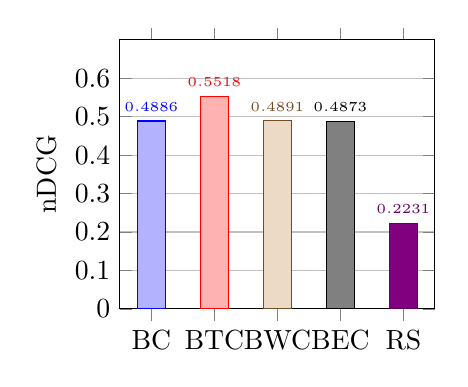
\begin{tikzpicture}
 \begin{axis}[
 	height=5cm,
 	width=4cm,
 	ybar =-10pt,
 	x = .8cm,
 	ymin=0.00, 
 	ymax=0.70,
 	ytick = {0,0.1,0.20,0.3,0.4,0.5,0.60},
 	scaled y ticks = false,
	enlarge x limits ={abs=.4cm},
	nodes near coords,
    every node near coord/.append style={font=\tiny,/pgf/number format/.cd,precision=4},
 	ylabel={nDCG},
	xtick={0,1,2,3,4},  % NEW BIT
	xticklabels={BC, BTC, BWC, BEC, RS},
	%legend style={at={(0.5,-0.1)},
	%anchor=north,legend columns=-1},
	ymajorgrids = true,]

		\addplot coordinates {(0,0.4886)};    
		\addplot coordinates {(1,0.5518)};    
		\addplot coordinates {(2,0.4891)};    
		\addplot coordinates {(3,0.4873)};    
		\addplot coordinates {(4,0.2231)};
        %\legend{BC, BTC, BWC, BEC, Random}
     \end{axis}
\end{tikzpicture}
\end{minipage}
\begin{minipage}{.46\textwidth}\centering
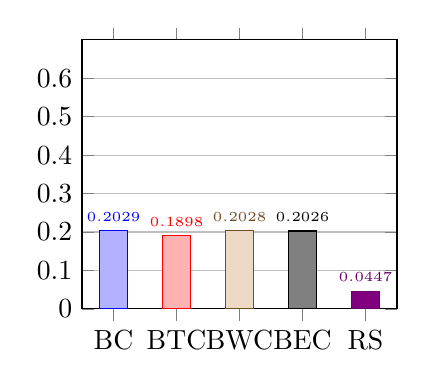
\begin{tikzpicture}
 \begin{axis}[
 	height=5cm,
 	ybar =-10pt,
 	x = .8cm,
 	ymin=0.0, 	
 	ymax=0.70,
 	ytick = {0,0.1,0.20,0.3,0.4,0.5,0.60},
	enlarge x limits ={abs=.4cm},
	nodes near coords,
    every node near coord/.append style={font=\tiny,/pgf/number format/.cd,precision=4},
	xtick={0,1,2,3,4},  % NEW BIT
	xticklabels={BC, BTC, BWC, BEC, RS},
	%legend style={at={(0.5,-0.1)},
	%anchor=north,legend columns=-1},
	ymajorgrids = true,]

		\addplot coordinates {(0,0.2029)};    
		\addplot coordinates {(1,0.1898)};    
		\addplot coordinates {(2,0.2028)};    
		\addplot coordinates {(3,0.2026)};    
		\addplot coordinates {(4,0.0447)};
        %\legend{BC, BTC, BWC, BEC, Random}
     \end{axis}
\end{tikzpicture}
\end{minipage}
\end{figure}
\end{frame}

\begin{frame}
	\frametitle{Possible Solutions}
	\begin{itemize}
		\item Calculate nDCG using the predicted ratings
		\item Ordering the individual ranked list by the average for the group
	\end{itemize}
\end{frame}
\chapter{Conclusion} \label{ch:conclusion}
We wanted to showcase an approach that reconciles the differences in preferences among multiple group members in the problem of group recommendation. During this process we found that the evaluation possibilities of the performance of these approaches were rather limited due to lack of proper datasets making it difficult to determine whether or not a group would be satisfied with its recommendations.

We found that with using a ranked list for the recommendations we could adopt the normalized Discounted Cumulative Gain(nDCG) technique from the information retrieval domain to measure user satisfaction by comparing the ranked list of a user with the ranked list found through aggregation. This only left us with the task of forming the groups, which we ended up doing using random sampling.

We sought to answer the following questions from the problem statement:
\begin{itemize}
	\item How to reflect group decision making algorithmically while securing satisfaction for the individuals as well as the group as a whole?
	\item How to measure the level of satisfaction in a group in regards to the items recommended?
	\item How to make recommendations to a group of people based on the users' individual preferences?
\end{itemize}

For reflecting how a group decision would be handled, we ventured into some of the methods used for resolving differing opinions. In the end, we incorporated single transferable vote into the Borda Count method in the Borda Transferable Count(BTC) algorithm. These are not methods that necessarily reflects an organic group decision process, but reflects parts of real group decision methodologies.

For measuring the level of satisfaction in a group, we found and used nDCG. It is commonly used for rankings and information retrieval. This works well with the view of recommendation as a tool for drawing out relevant information, when getting an overview is hard.

For making recommendations to a group, we present the BTC as a method of aggregating the individual ranked lists. The results are promising, as it performs better than the tested methods on nDCG scores. However, we cannot as of yet make a definite conclusion on the BTC as a solution to the group recommender problem.

\section{Discussion}\label{sec:conclusion_discussion}
As mentioned we use the information retrieval method nDCG to measure satisfaction. In doing so we make several assumptions about the users’ preferences. First of all, the user ratings used for the group recommendations are predictions, which may not coincide with the actual preferences of the user. Based on these predicted ratings we assume that a user would construct a ranked list, with a fixed distance between the top ranked and next highest rank regardless of the predicted preference for either, which we use to determine the satisfaction score, with the highest ratings. This means that the satisfaction score we get is based on assumptions about a user's preferences, which makes our results noteworthy, but ultimately, based on assumptions about existing data rather than real world data.

In order for us to get a concrete result we need to measure satisfaction with real users as to prove the effectiveness of the method presented in this project. Provided that, the method could point in the direction that group recommendation is a voting problem.

\bibliographystyle{ACM-Reference-Format}
\bibliography{references} 

\begin{appendices}
\section{Survey}
%Context about why we needed the data

%How the whole thing went down
In order to make a dataset in a short time frame, we looked into crowdsourcing, where it was possible to pay people to answer surveys or do tasks that computers cannot. In particular we were looking at Clickworker and Mechanical Turk, which allowed external surveys. Since no sites had an inbuilt survey creation tool that could handle our requirements, we decided to make our own survey website.

Using this method, we could potentially reach thousands of people without limiting us to the survey tools made available on the standard websites.

%Creation of the website
For web hosting, we went to DigitalOcean, which offered a Ubuntu server setup with Django. We added Gunicorn as the WSG interface and nginx as the http server. Behind it all, we had a MySql database keeping track of the survey questions and results along with timestamps.

%Django as Python web application framework
%Gunicorn as Web Server Gateway Interface(WSGI) server. A traditional web server does not understand or have any way to run Python applications. WSGI is a standard interface for py modules and containers.
%Digical Ocean as webhost with Unix as the OS
%MySql as the database

%The survey
The survey itself asks participants to personally give a recommendation to a group of users. The participant knows each user's own top 10 preference, and must decide on their own what aggregation strategy they wish to follow. An important aspect of the survey was making it as easy to complete as possible. As we had to pay each participant, each such improvement could be translated to a saving, which in turn translated to a larger and more useful dataset. So to make it more intuitive and not overload each user with information, we made it so that hovering the mouse over a movie title will make the movie's position light up on all the other users' rankings, shown in Figure \ref{fig:appendix_userprefs}, and gave the user a tooltip about other movie positions. Additionally, we made the ranking system into a drag-and-drop, such that the participant could drag and easily rearrange their recommendations. This can be seen in Figure \ref{fig:appendix_recbox}.

\begin{figure}\label{fig:appendix_recbox}
	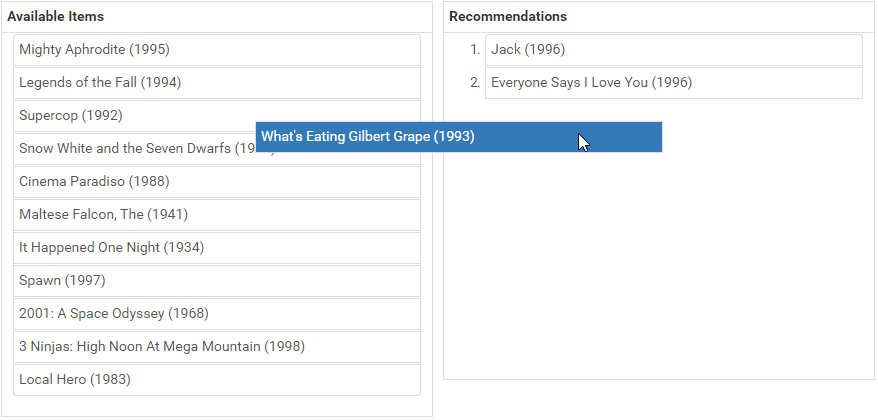
\includegraphics[scale=0.35]{graphics/recbox.png}
	\caption{The list of available items and the box holding the recommendations of the survey participant}
\end{figure}

\begin{figure}\label{fig:appendix_userprefs}
	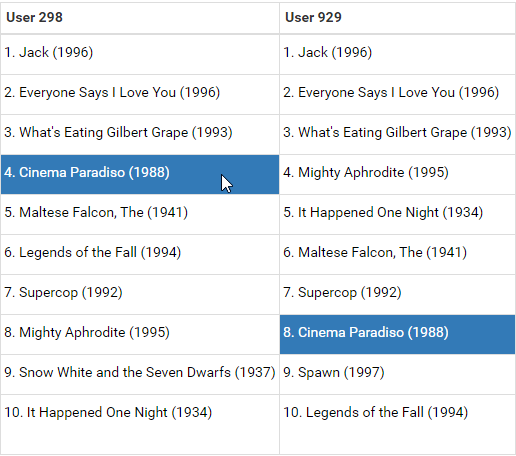
\includegraphics[scale=0.5]{graphics/users.png}
	\caption{Two lists of movie preferences for a user}
\end{figure}

After making a recommendation, the user could proceed to the next step, and upon completing all steps they would reach a screen providing them with a code. With each step, the group size is increased by one, going from 4 to 8 users. The code is important, as the participant must present this as evidence to the crowdsourcing site as proof of their participation. For our survey, we decided to generate a unique code for each participant mixing the assigned groups and a timestamp, so that we could deduce which user responded when and with what. This precaution was necessary so that it was possible to filter out participants rushing through the survey with no care for their answers.

Also, since we wanted to have a balanced dataset, we separated our groups into 40 sets of groups of size 4 to 8, and made it so that every user would get a randomly picked set. The database would keep track of how many responses each set had, such that we could prioritize the sets with fewer responses and get a balanced dataset. It would also mean that anyone taking the test twice would be unlikely to see the same survey.

Before running the survey on Mechanical Turk, we ran it past some other willing participants for evaluation and decided to halve the number of groups each participants would give recommendations to from 10 to 5, due to feedback about the length of the survey. \note{This section can be expanded to better reflect the process and changes happening to the survey, as a lot of work went into it in the project}

%Most importantly, we realized how vital it was to make the par

%Dealing with mechanical turk
For the crowdsourcing website, we ended up going with Amazon's Mechanical Turk, as it is the more well-known and cheaper service. When ready, we injected a good amount of money on the account, as one had to prepay for any work requested and started up a limited run to test out the services and find a suitable price range. We managed to get a few responses. On Mechanical Turk, the participant would see our survey, click in and be provided a link to our survey. Upon completion of the survey, our participant would get the code and input it on the Mechanical Turk website. Initial results were interesting with big differences between how much time participants spent on the survey. We noted a few obvious cheaters who blazed through a survey in seconds thanks to the timestamps, however as a requester and with the timestamps in our database, we would be able to sort them out, and we could also reject their work on the Mechanical Turk site.

Though, on the third day of this limited run we ran into problems with Amazon Mechanical Turk. We were unable to access our account, and had to contact their support team. Soon enough the support team responded that our account had been suspended, and that we would be informed about the reason for the suspension in 2-3 days along with fate of our account. In two days time, Mechanical Turk support wrote us that our account had been suspended indefinitely and our current survey stopped because of a violation of the participation agreement. Unaware of any possible violations we could have made, we made further inquires, but never got a clear answer. Additionally, our funds on the account were also confiscated. So in the end, we ended up only getting responses totaling a few dollars worth of data.

%Show data and evaluate on them.
\end{appendices}

\end{document}
